\documentclass[10pt]{beamer}
\usetheme[progressbar=frametitle]{metropolis}
\usepackage{appendixnumberbeamer}
\usepackage{booktabs}
\usepackage[scale=2]{ccicons}
\usepackage{pgfplots}
\usepgfplotslibrary{dateplot}
\usepackage{xspace}
\usepackage{bm}
\usepackage{graphicx}
\usepackage{subcaption}
\usepackage{anyfontsize}
\metroset{block=fill}

\title{Gaussian Processes}
\subtitle{Definition, applications and deep extension}
\date{\today}
\author{Luis Antonio Ortega Andrés}
%\institute{}
% \titlegraphic{\hfill\includegraphics[height=1.5cm]{logo.pdf}}

\begin{document}

\maketitle

\begin{frame}{Table of contents}
  \setbeamertemplate{section in toc}[sections numbered]
  \tableofcontents%[hideallsubsections]
\end{frame}

\section[Definitions]{Definition}

\begin{frame}[fragile]{Gaussian process}

    \begin{alertblock}{Gaussian process}
        A \textbf{Gaussian process} is a \textbf{stochastic process}, i.e, a collection of random variables \( \{X_t\}_{t\in \mathcal{T}} \) indexed by a set $\mathcal{T}$, such that any finite subset is Gaussian.
        
        \[
             \{X_{t_1}, \dots, X_{t_N}\} \sim \mathcal{N}\left(\cdot, \cdot\right)
        \]
    \end{alertblock}
\end{frame}

\begin{frame}
    \centering
    For example, \( X_{t_i} \sim \mathcal{N}( \cdot, \cdot) \). 

    \centering    
    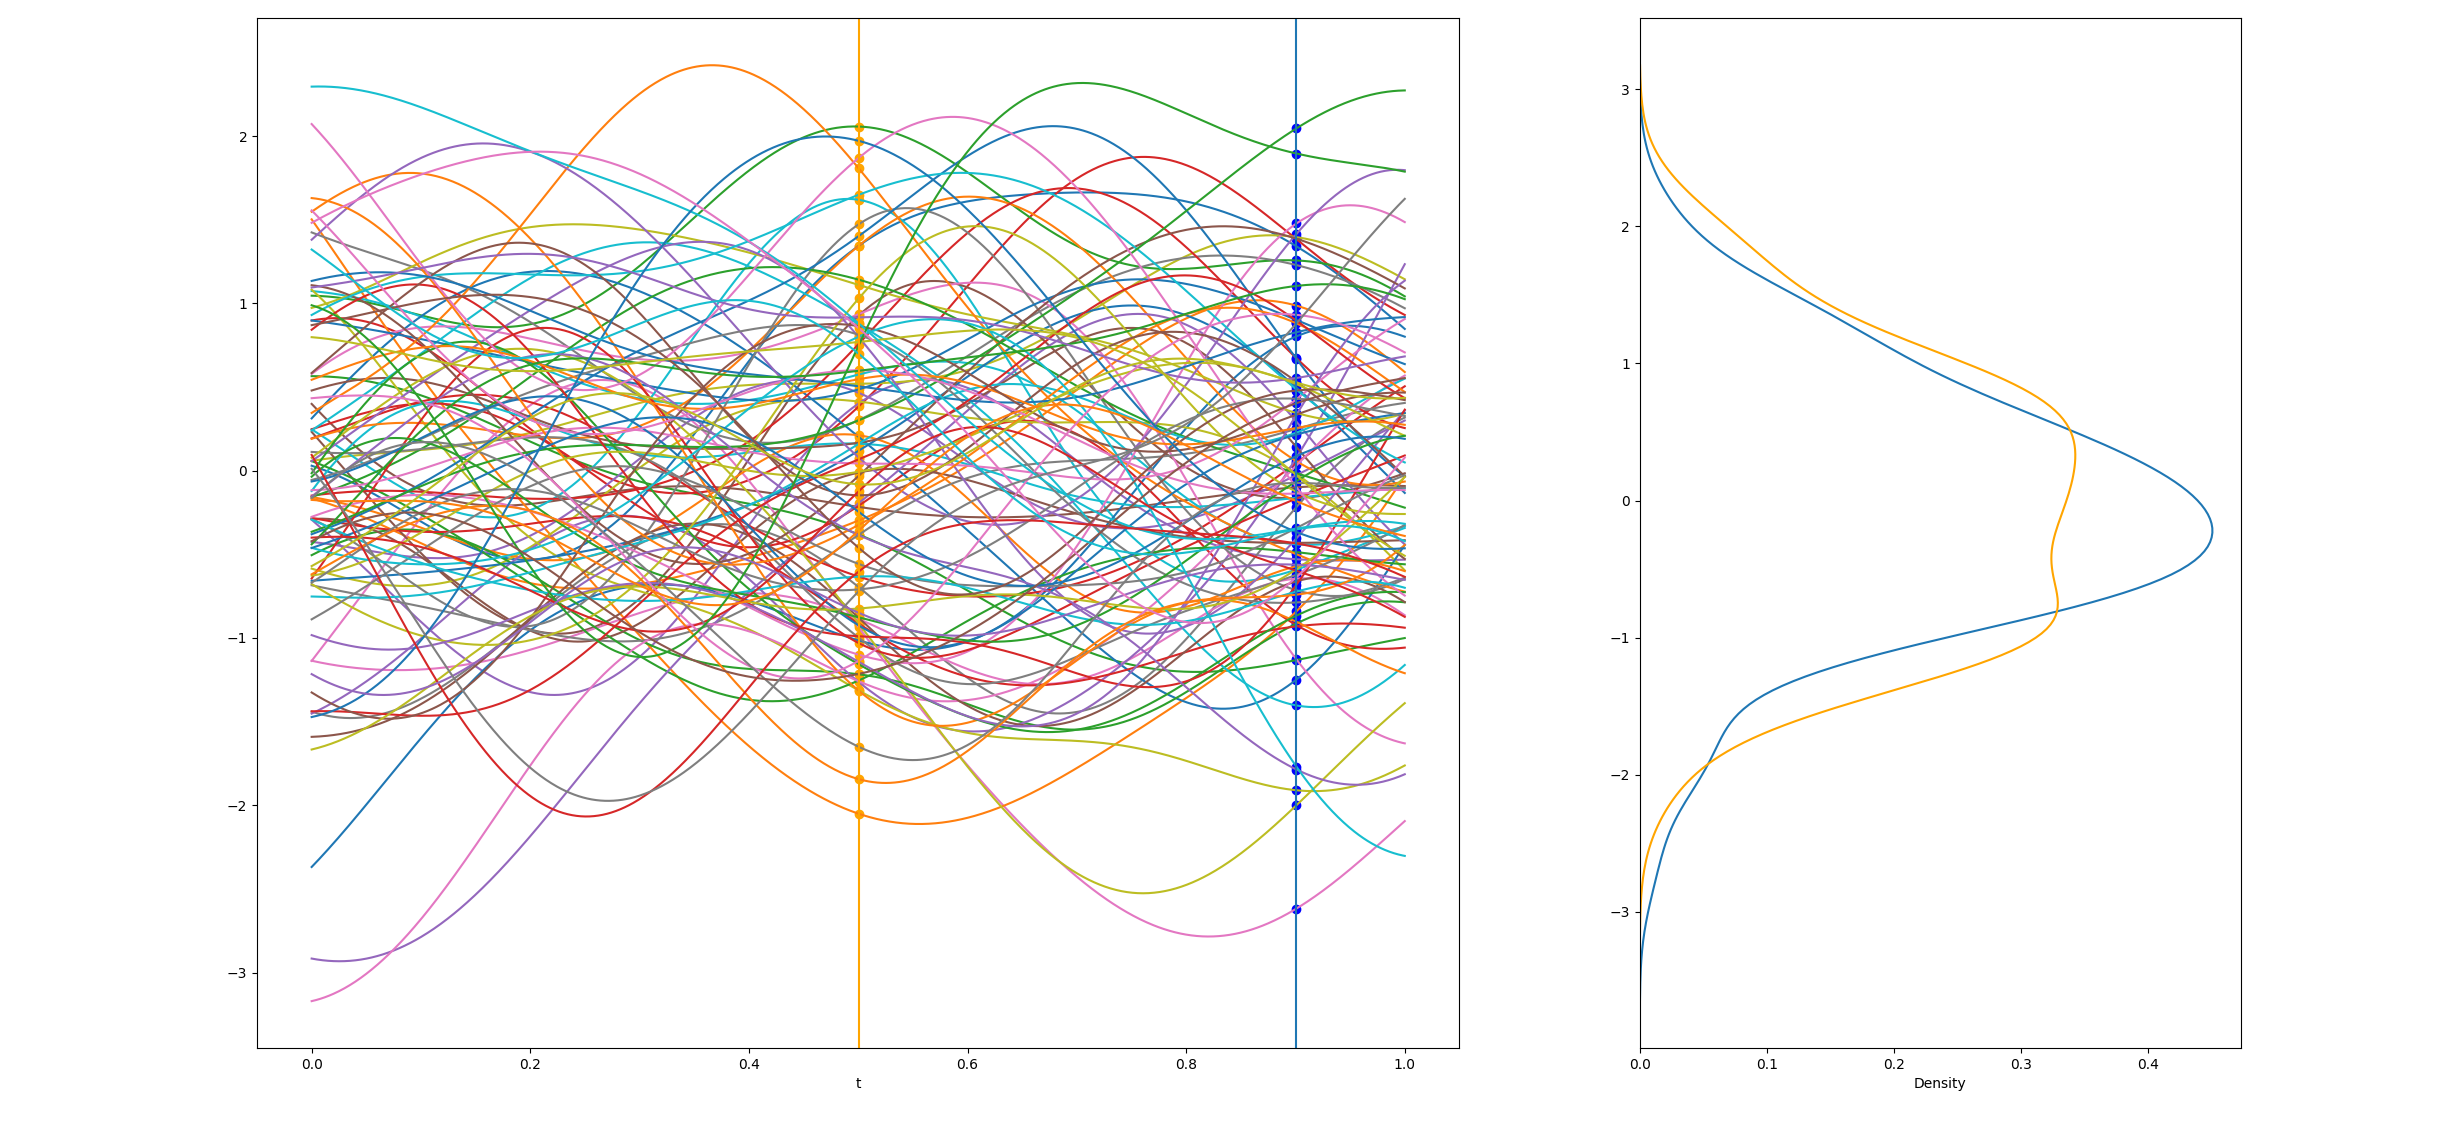
\includegraphics[scale = 0.17]{imgs/GP_intro.png}

\end{frame}

\subsection{Characterization}
\begin{frame}{Characterization}
    Gaussian processes are completely determined by their first and second order moments\footnote{Bishop, Christopher M. Pattern recognition and machine learning. Springer, 2006.}.

    Given \( \bm{t} = (t_1, \dots, t_N) \), \( N \in \mathbb{N} \):
    \[
         X(\bm{t}) = (X_{t_1}, \dots, X_{t_N}) \sim \mathcal{N}\left( m(\bm{t}), K(\bm{t}, \bm{t}) \right)
    \] 
    \[
         \text{ where } 
         \begin{cases}
             m(\bm{t}) &= \mathbb{E}\left[X(\bm{t})\right]\\
             K(\bm t, \bm t) &= Cov\left(X(\bm{t}), X(\bm{t})\right)
         \end{cases}
    \] 
    
    Defining \( m \) and \( K \) we get a Gaussian process.
\end{frame}

\subsection{Examples}
\begin{frame}{Examples}
    It is usual to take a \textbf{zero mean function}, \( m(\bm{t}) = 0 \) and \textbf{kernel functions}:
    \begin{itemize}
        \item \textit{RBF}: \( K (\bm{t}, \bm{t}') = \exp \left( - \frac{\|\bm t - \bm t' \|^{2}}{2\sigma^{2}} \right) \). 
        \item \textit{Matérn}: Family of kernels, parameterized by \( \nu \). Generalize several kernels. 
    \end{itemize} 

    \centering
    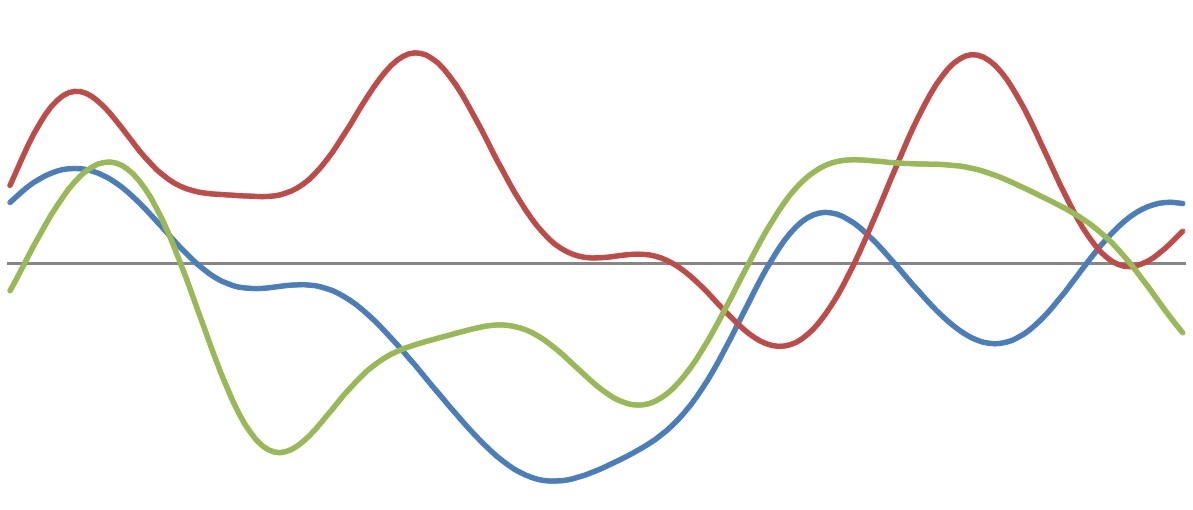
\includegraphics[scale = 0.2]{imgs/GP.png}

    Define a \textbf{probability distribution over functions}: \emph{Given a function, which is its probability when interpreted as a sample of a Gaussian process?}
\end{frame}

\section{Regression Problem}
\begin{frame}{Problem statement}
    Given dataset \( \mathcal{D} = \{(\bm x_1, y_1), \dots, (\bm x_N, y_N)\} \) and an unknown function \( f \) such that
    \[
         y_n = f(\bm x_n) + \epsilon\quad \forall n=1,\dots,N, \quad \text{where} \quad \epsilon \sim \mathcal{N}(0, \sigma^2)
    \] 

    \begin{alertblock}{Assumption}
            Function \( f \) is a Gaussian process of unknown mean function \( m \) and kernel function \( K \)
    \end{alertblock}
\end{frame}


\begin{frame}
    \begin{alertblock}{Assumption}
    Function \( f \) is a Gaussian process of unknown mean function \( m \) and kernel function \( K \)
    \end{alertblock}

    \centering
    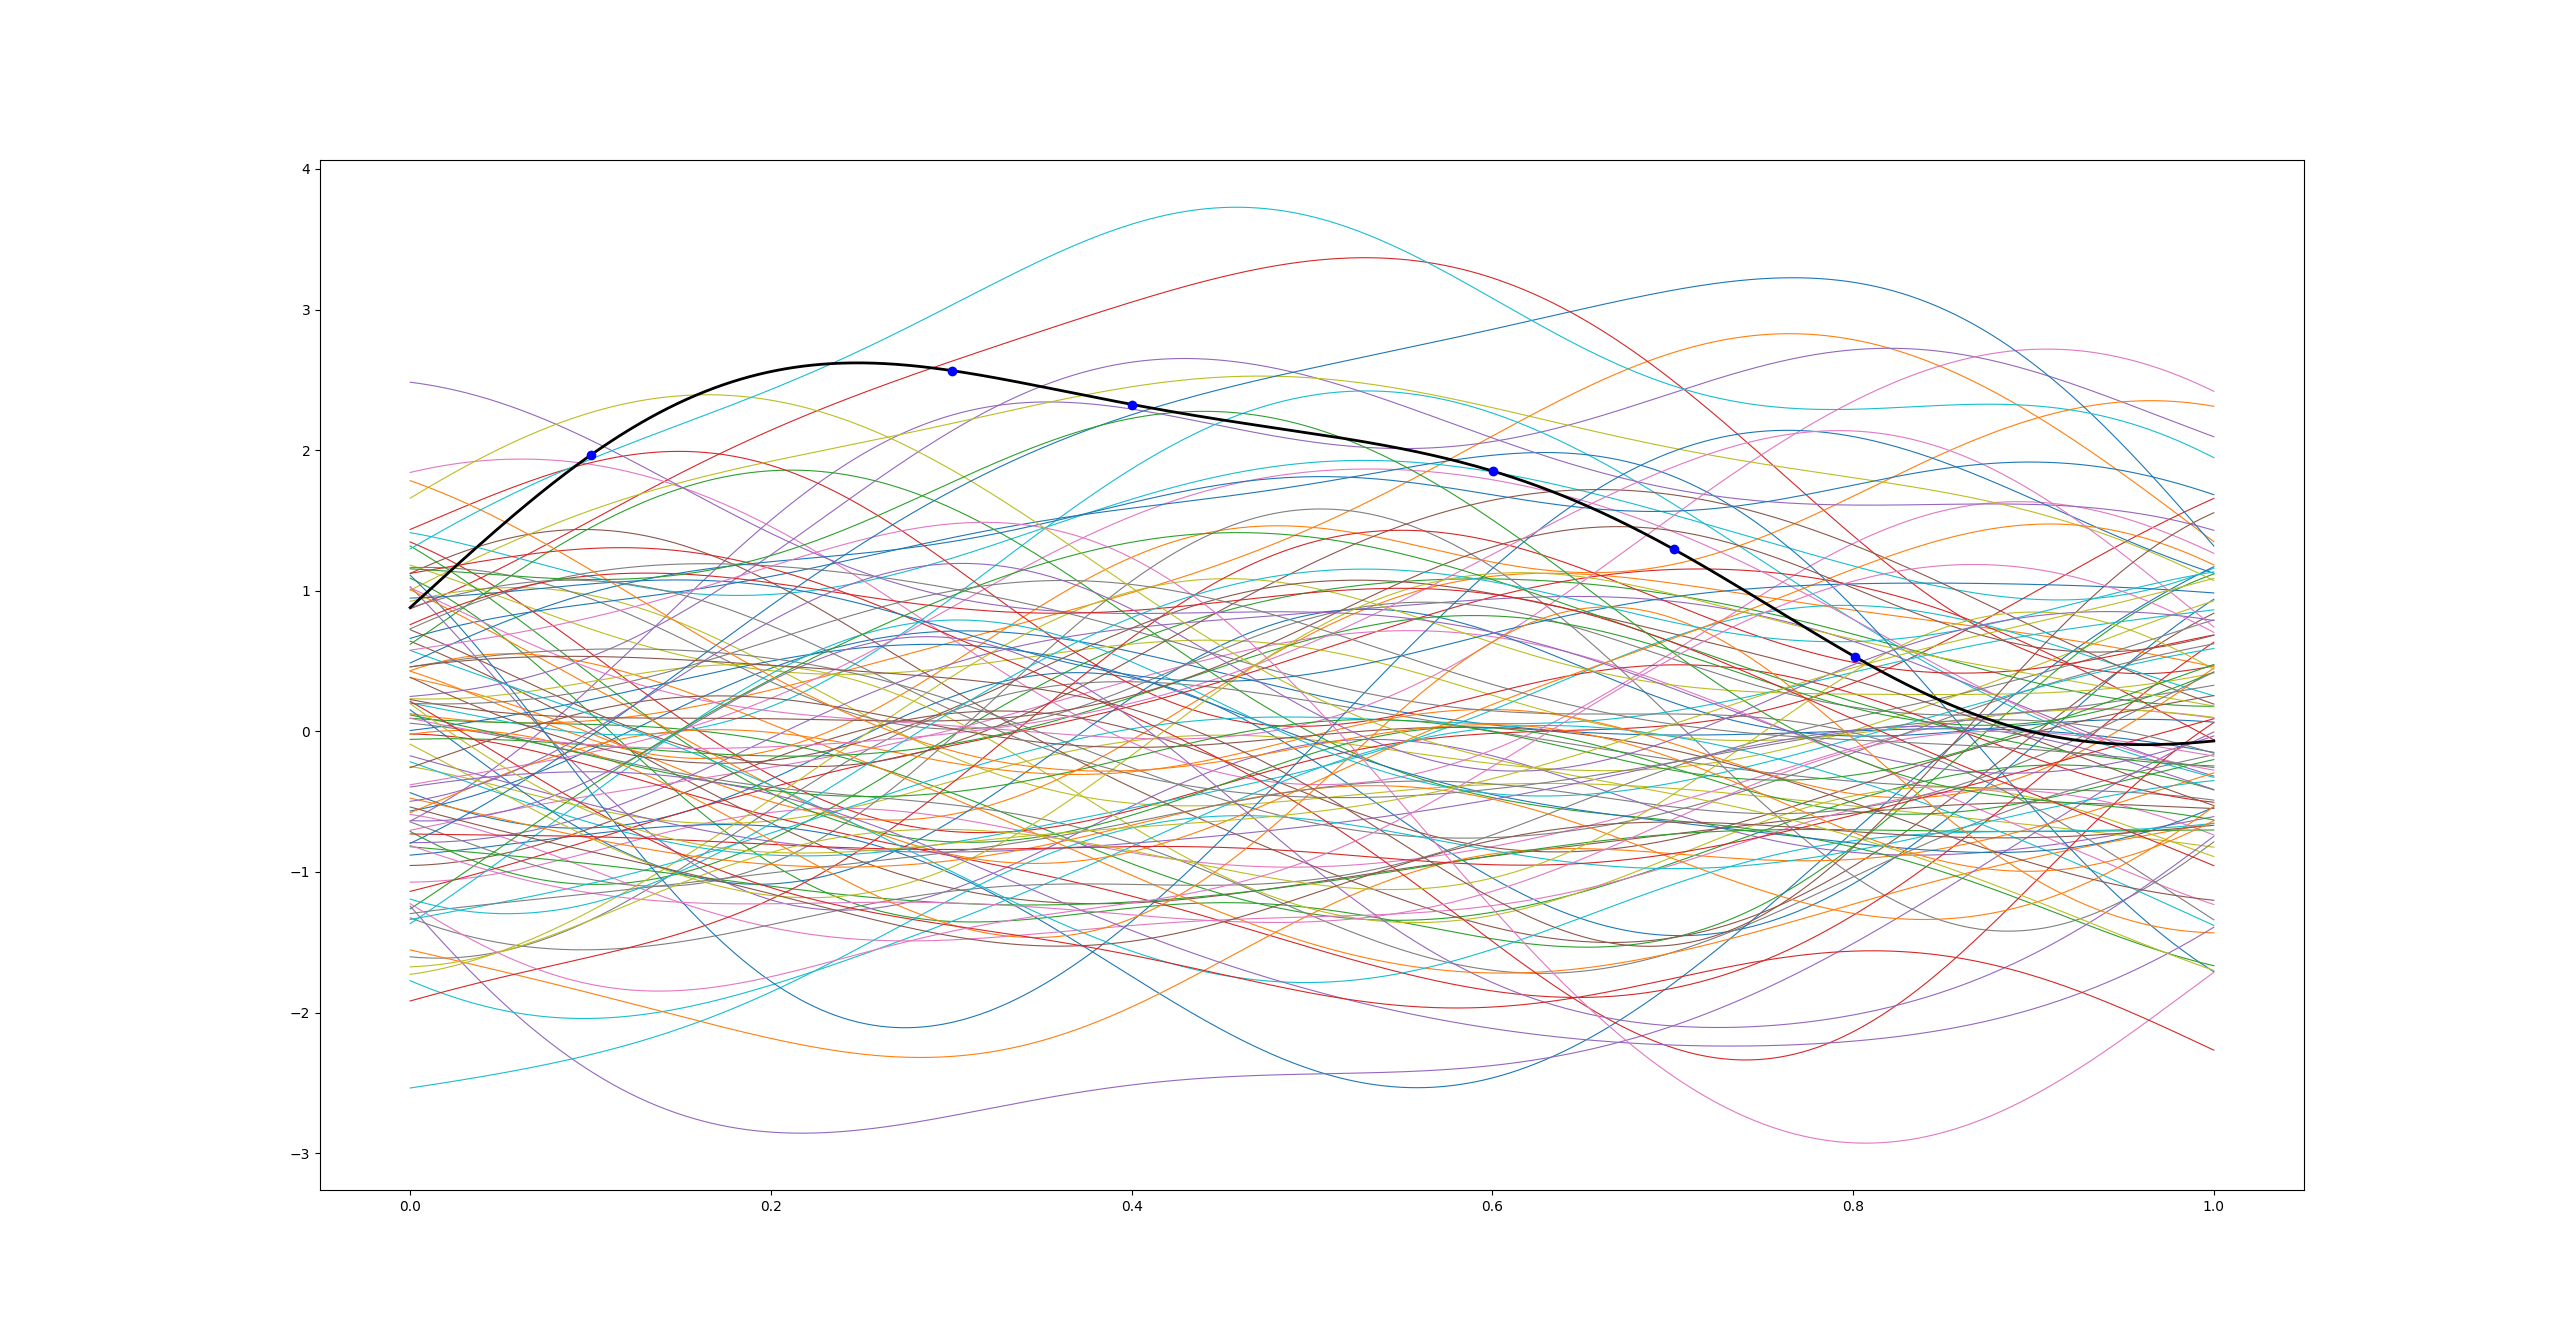
\includegraphics[scale=0.17]{imgs/funct_as_gp.png}
\end{frame}



\begin{frame}
    Naming \( \bm{X} = (\bm{x}_1, \dots, \bm{x}_N) \) and \( \bm{y} = (y_1,\dots, y_N) \):
    \[
         \bm{y} = f(\bm{X}) + \mathcal{N}(0, \sigma^2 \bm{I}) \implies \bm{y} \sim \mathcal{N}\left( m(\bm{X}), K(\bm{X}, \bm{X}) + \sigma^2\bm{I} \right).
    \]

    Remark: \emph{A distribution is assumed over function points} \textbf{but not over} \( x \).

    Let \( \bm{X}^* \) be a test case where \( \bm{y}^* =  f(\bm{X}^*) + \mathcal{N}(0, \sigma^2 \bm{I})\):
    \[
         \begin{pmatrix} f(\bm{X}) \\ f(\bm{X}^*) \end{pmatrix} \sim \mathcal{N}\left( 
             \begin{pmatrix}
             m(\bm{X}) \\ m(\bm X^*)
         \end{pmatrix}, \begin{pmatrix}
             K ( \bm{X} , \bm X) & K(\bm X, \bm X^*) \\
             K (\bm X^*, \bm X) & K (\bm X^*, \bm X^*)
         \end{pmatrix} \right)
    \]
    
    An \textbf{usual assumption} is that \( m = 0 \). 

    \begin{alertblock}{\textcolor{black}{Remark}}
        Typically, \( \bm x \) is erased from the notation.
    \end{alertblock}
\end{frame}


\begin{frame}
    Naming \( \bm{X} = (\bm{x}_1, \dots, \bm{x}_N) \) and \( \bm{y} = (y_1,\dots, y_N) \):
    \[
         \bm{y} = \textcolor{orange}{\bm{f}} + \mathcal{N}(0, \sigma^2 \bm{I}) \implies \bm{y} \sim \mathcal{N}\left( \textcolor{blue}{0}, \textcolor{orange}{\bm K_{\bm f, \bm{f}}} + \sigma^2\bm{I} \right).
    \]

    Remark: \emph{A distribution is assumed over \( \bm f \)  points} \textbf{but not over} \( \bm X \).

    Let \( \bm{X}^* \) be a test case where \( \bm{y}^* = \textcolor{orange}{\bm{f}^*} + \mathcal{N}(0, \sigma^2 \bm{I})\):
    \[
         \begin{pmatrix} \textcolor{orange}{\bm{f}} \\ \textcolor{orange}{\bm{f}^*} \end{pmatrix} \sim \mathcal{N}\left( 
             \textcolor{blue}{0}, \begin{pmatrix}
            \textcolor{orange}{\bm K_{\bm f, \bm f}} & \textcolor{orange}{\bm K_{\bm f, \bm f^*}} \\
            \textcolor{orange}{\bm K_{\bm f^*, \bm f}} & \textcolor{orange}{\bm K_{\bm f^*, \bm f^*}}
         \end{pmatrix} \right)
    \]
\end{frame}



\begin{frame}{Predictive posterior}
    \[
        \begin{pmatrix} \bm f \\ \bm f^* \end{pmatrix} \sim \mathcal{N}\left(\bm{0}, \begin{pmatrix}
            \bm K_{\bm f, \bm f} & \bm K_{\bm f, \bm f^*} \\
            \bm K_{\bm f^*, \bm f} &\bm K_{\bm f^*, \bm f^*}
         \end{pmatrix} \right) \quad
        \bm{y} \mid \bm f \sim \mathcal{N}( \bm f, \sigma^2\bm{I})
    \]
    \[
         \Downarrow
    \]
    \[
        P(\bm y \mid \bm f, \bm f^*) = P(\bm y \mid \bm f) \implies \bm y \mid \bm f, \bm f^* \sim \mathcal{N}(\bm f, \sigma^2 \bm I)
    \]
    \[
         \Downarrow
    \]
    \[
         \bm f, \bm f^* \mid \bm y \sim \mathcal{N}(\cdot, \cdot) \implies \bm f^* \mid \bm y \sim \mathcal{N}(\cdot, \cdot)
    \]
    \[
         \Downarrow
    \]
    \[
         \bm f^* \mid \bm{y} \sim \mathcal{N}(\bm{\mu}, \bm{\Sigma}) \quad
         \begin{cases}
         \bm \mu = \bm K_{\bm f^*, \bm f}(\bm K_{\bm f, \bm f} + \sigma^2\bm I)^{-1}\bm y\\
         \bm{\Sigma} = \bm K_{\bm f^*, \bm f^*} - \bm K_{\bm f^*, \bm f}(\bm K_{\bm f, \bm f}   + \sigma^2 \bm I)^{-1} \bm K_{\bm f, \bm f^*} 
         \end{cases}
    \]

\end{frame}

\begin{frame}
    \begin{figure}
        \centering
        \begin{subfigure}[b]{0.475\textwidth}
            \centering
            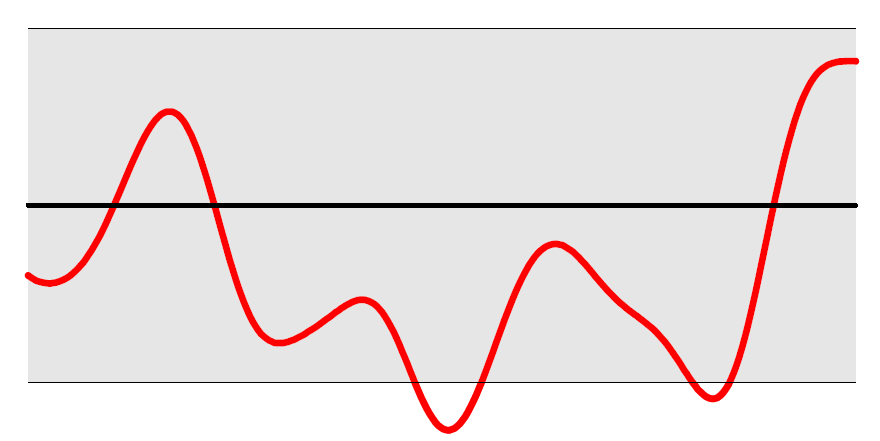
\includegraphics[width=\textwidth]{imgs/GP_1}
        \end{subfigure}
        \hfill
        \begin{subfigure}[b]{0.475\textwidth}  
            \centering 
            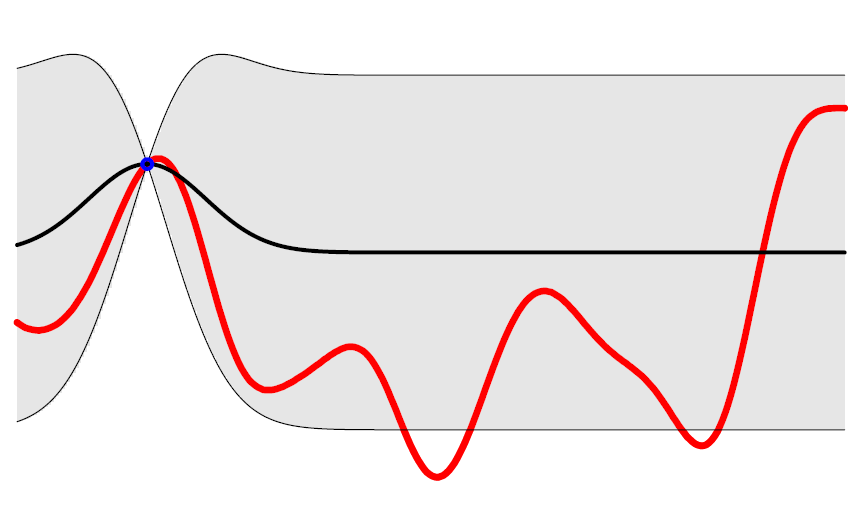
\includegraphics[width=\textwidth]{imgs/GP_2}
        \end{subfigure}
        \vskip\baselineskip
        \begin{subfigure}[b]{0.475\textwidth}   
            \centering 
            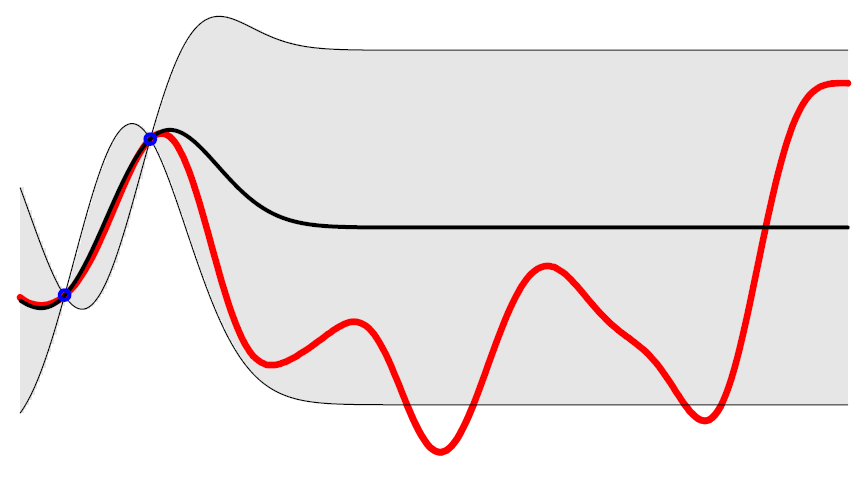
\includegraphics[width=\textwidth]{imgs/GP_3}
        \end{subfigure}
        \hfill
        \begin{subfigure}[b]{0.475\textwidth}   
            \centering 
            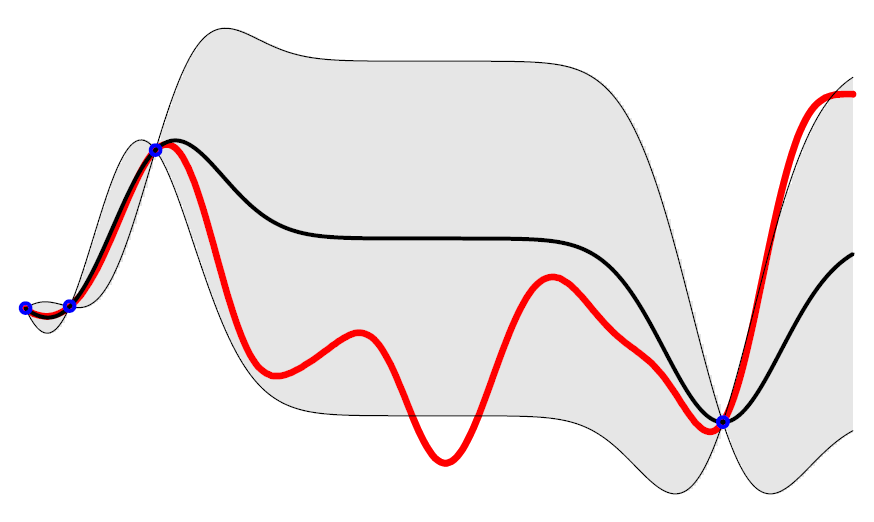
\includegraphics[width=\textwidth]{imgs/GP_4}
        \end{subfigure}
    \end{figure}
\end{frame}

\begin{frame}

    Unknown function \( f(x) = \sin(x) \), \( \mathcal{D} \) is a sample of \( 8 \) points in \( (-5, 5) \), RBF kernel.

    \centering
    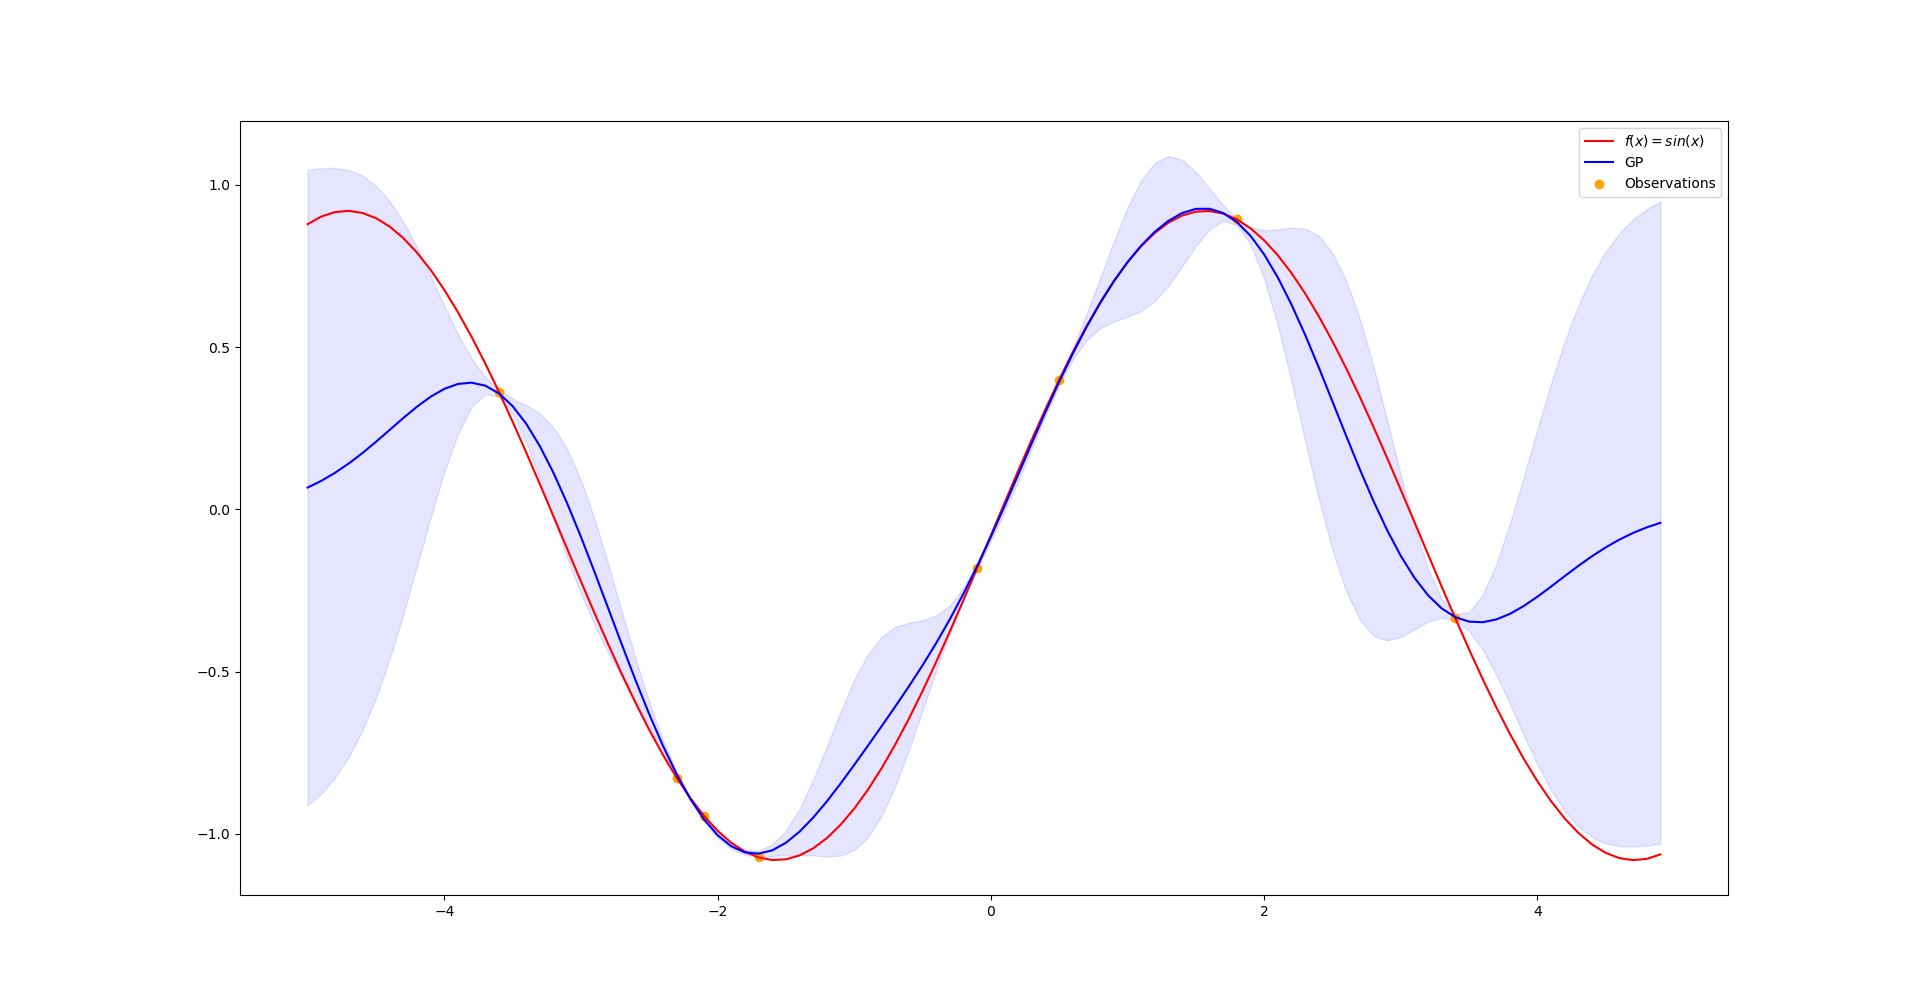
\includegraphics[scale = 0.2]{imgs/GP_post.png}
\end{frame}

\subsection{Computational complexity}
\begin{frame}{Computational complexity}
    Several computations are done, assuming \( \bm X \) has \( N \) points and \( \bm X^* \) has \( M \):
    \[
         \begin{aligned}
             \bm K_{\bm f, \bm f} &\implies \mathcal{O}(N^2)\\
             \left(\bm K_{\bm f, \bm f} + \sigma^2 \bm I \right)^{-1} &\implies \mathcal{O}(N^3)\\
             \bm K_{\bm f, \bm f^*} = \bm K_{\bm f^*, \bm f}^T &\implies \mathcal{O}(NM)\\
             \bm K_{\bm f^*, \bm f^*} &\implies \mathcal{O}(M^2)\\
         \end{aligned}
    \] 

Training: \( \mathcal{O}(N^3) \) and Test: \( \mathcal{O}(NM^2) \). They are \textbf{computationally inefficient!!}  

This can be slightly reduced using the \emph{Cholesky decomposition} for the matrix inversion.
\end{frame}

\begin{frame}{Advantages}
    They give a prediction \( \bm \mu =\bm K_{\bm f^*, \bm f}(\bm K_{\bm f, \bm f} + \sigma^2\bm I)^{-1}\bm y\). \textbf{Equals the kernel ridge regression estimator!!}.   

    Implicit \textbf{confidence interval}, \( (\bm \mu - 3\bm \Sigma, \bm \mu + 3\bm \Sigma) \). 

    Full \textbf{probabilistic approach}.
\end{frame}

\section{Inducing points}

\begin{frame}{Inducing points}
        
    \textbf{Main idea}: Use a \emph{smaller} and \emph{hidden} set of points.

    Let \( \bm{X}_u \subset \mathbb{R}^D\) be a set of \emph{known} points (commonly computed from \( \bm{X} \)). We make the assumption that \( \bm{u} = f(\bm{X}_u) \) is representative of \( \bm{y} \).

    \textbf{Remark.} The \emph{inducing points} \( \bm u \) are \emph{unknown} and must be \emph{marginalized}.
    \[
        \begin{aligned}
         P(\bm f, \bm f^*) &= \int P(\bm f, \bm f^*, \bm u) \ d\bm u\\
         &= \underbrace{\int P(\bm f, \bm f^* \mid \bm u) P(\bm u) \ d\bm u}_{Intractable}
        \end{aligned}
        \qquad
        \raisebox{-15mm}{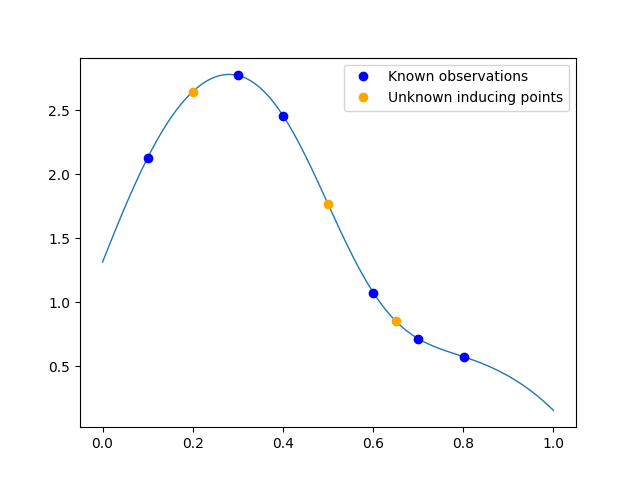
\includegraphics[keepaspectratio = true, scale = 0.3]{imgs/ind_p.png}}
    \]


    Where \( \bm{u} \) are taken from a Gaussian process:
    \[
         \bm{u} \sim \mathcal{N}(0, \bm K(\bm{X}_u, \bm{X}_u)).
    \]
\end{frame}

\begin{frame}{Approaches}
    \begin{itemize}
        \item Exact inference in approximated model:
        \[
             P( \bm f, \bm f^* \mid \bm u) = P\left( \bm f \mid \bm u)\ P( \bm f^* \mid \bm u\right)
        \]
        \[
             \Downarrow
        \]
        \[
            P(\bm f, \bm f^*) = \int P( \bm f \mid \bm u)\ P( \bm f^* \mid \bm u) \ P(\bm u) \ d\bm u
        \]
        And further approximate \(  P( \bm f \mid \bm u) \) and \(  P( \bm f^* \mid \bm u) \)  
        \item Variational inference:
        \[
             Q(\bm{u}) \approx P(\bm{u} \mid \bm{y}).
        \]
    \end{itemize}
\end{frame}

\begin{frame}{Approximated models}
    \begin{alertblock}{\textcolor{black}{Exact conditionals}}
    \[
        \begin{aligned}
         P(\bm f \mid \bm u) &= \mathcal{N}(\bm K_{\bm f, \bm u}\bm K_{\bm u, \bm u}^{-1} \bm u, \bm K_{\bm f, \bm f} - \bm Q_{\bm f, \bm f} )\\
         P(\bm f^* \mid \bm u) &= \mathcal{N}(\bm K_{\bm f^*, \bm u}\bm K_{\bm u, \bm u}^{-1} \bm u, \bm K_{\bm f^*, \bm f^*} - \bm Q_{\bm f^*, \bm f^*})\\
        \bm Q_{\bm a, \bm b} &= \bm K_{\bm a, \bm u} \bm K_{\bm u, \bm u}^{-1} \bm K_{\bm u, \bm b}
        \end{aligned}
    \]
    \end{alertblock}
    \begin{itemize}
        \item The Subset of Regressors approximation
            \[
                \begin{aligned}
                 Q_{SOR}(\bm f \mid \bm u) &= \mathcal{N}(\bm K_{\bm f, \bm u}\bm K_{\bm u, \bm u}^{-1} \bm u, 0 )\\
                 Q_{SOR}(\bm f^* \mid \bm u) &= \mathcal{N}(\bm K_{\bm f^*, \bm u}\bm K_{\bm u, \bm u}^{-1} \bm u, 0)
                \end{aligned}
            \]
        \item The Deterministic Training Conditional approximation 
            \[
                \begin{aligned}
                 Q_{DTC}(\bm f \mid \bm u) &= \mathcal{N}(\bm K_{\bm f, \bm u}\bm K_{\bm u, \bm u}^{-1} \bm u, 0 )\\
                 Q_{DTC}(\bm f^* \mid \bm u) &= P(\bm f^* \mid \bm u)
                \end{aligned}
            \]
    \end{itemize}
\end{frame}

\begin{frame}
    \begin{alertblock}{\textcolor{black}{Exact conditionals}}
    \[
        \begin{aligned}
         P(\bm f \mid \bm u) &= \mathcal{N}(\bm K_{\bm f, \bm u}\bm K_{\bm u, \bm u}^{-1} \bm u, \bm K_{\bm f, \bm f} - \bm Q_{\bm f, \bm f} )\\
         P(\bm f^* \mid \bm u) &= \mathcal{N}(\bm K_{\bm f^*, \bm u}\bm K_{\bm u, \bm u}^{-1} \bm u, \bm K_{\bm f^*, \bm f^*} - \bm Q_{\bm f^*, \bm f^*})\\
        \bm Q_{\bm a, \bm b} &= \bm K_{\bm a, \bm u} \bm K_{\bm u, \bm u}^{-1} \bm K_{\bm u, \bm b}
        \end{aligned}
    \]
    \end{alertblock}
    \begin{itemize}
        \item The Fully Independent Training Conditional approximation 
            \[
                \begin{aligned}
                 Q_{FITC}(\bm f \mid \bm u) &= \mathcal{N}(\bm K_{\bm f, \bm u}\bm K_{\bm u, \bm u}^{-1} \bm u, diag(\bm K_{\bm f, \bm f} - \bm Q_{\bm f, \bm f}) )\\
                 Q_{FITC}(\bm f^* \mid \bm u) &= P(\bm{f}^* \mid \bm u)
                \end{aligned}
            \]
        \item The Partially Independent Training Conditional approximation
            \[
                \begin{aligned}
                 Q_{PITC}(\bm f \mid \bm u) &= \mathcal{N}(\bm K_{\bm f, \bm u}\bm K_{\bm u, \bm u}^{-1} \bm u, blockdiag(\bm K_{\bm f, \bm f} - \bm Q_{\bm f, \bm f}) )\\
                 Q_{PITC}(\bm f^* \mid \bm u) &= P(\bm{f}^* \mid \bm u)
                \end{aligned}
            \]
    \end{itemize}
\end{frame}

\begin{frame}{Variational bounds}
    Using Jensen's inequality:
    \[
         \log P(\bm y \mid \bm u) = \log \mathbb{E}_{P(\bm f \mid \bm u)}[P(\bm u \mid \bm f)] \geq  \mathbb{E}_{ \log P(\bm f \mid \bm u)}[P(\bm u \mid \bm f)] \equiv \mathcal{L}_1,
    \]
    raises Titsias' bound \footnote{Titsias, Michalis. ``Variational learning of inducing variables in sparse Gaussian processes.'' In Artificial intelligence and statistics, 2009.}
    \[
         \log P(\bm y) = \log \int P(\bm y \mid \bm u)P(\bm u) d\bm u \geq \log \int \exp \mathcal{L}_1 P(\bm u) d\bm u \equiv \mathcal{L}_2.
    \]
    But it is not suitable for \textbf{stochastic optimization}. Appears a new bound\footnote{Hensman, James, Nicolo Fusi, and Neil D. Lawrence. "Gaussian processes for big data." 2013. }
    \[
         \log P(\bm y) \geq \mathbb{E}_{Q(\bm u)}\left[\mathcal{L}_1 + \log P(\bm u) - \log Q(\bm u)\right] \equiv \mathcal{L}_3.
    \]
\end{frame}

\section{Deep Gaussian processes}

\begin{frame}{General idea}
    \textbf{Connect Gaussian processes in a chain.}
    \centering
    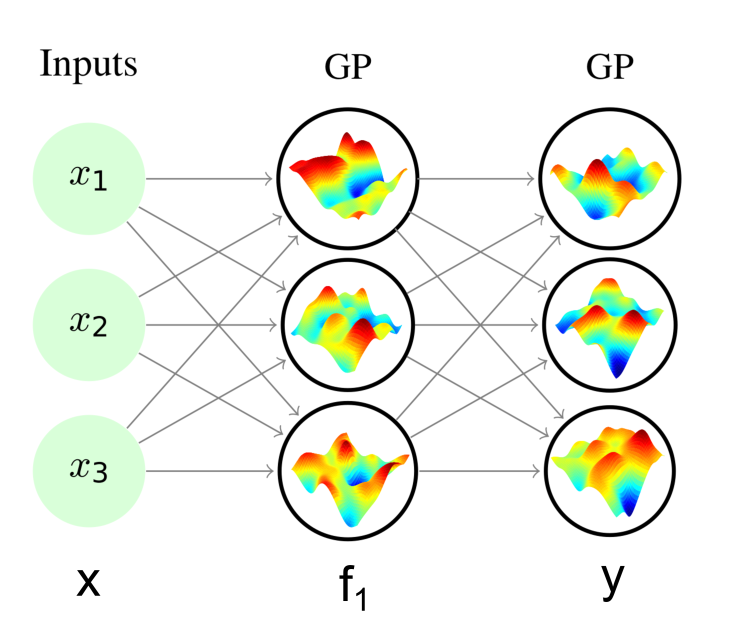
\includegraphics[scale = 0.17]{imgs/Deep_gp.png}\footnote{Image reference: https://www.groundai.com/project/inference-in-deep-gaussian-processes-using-stochastic-gradient-hamiltonian-monte-carlo/1}

    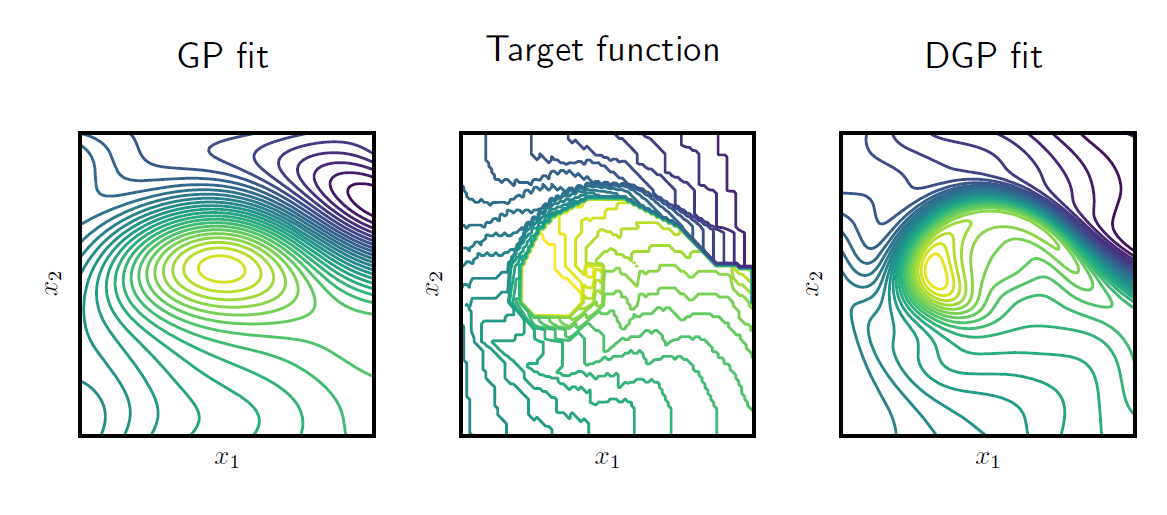
\includegraphics[scale = 0.2]{imgs/Deep_gp_fit.PNG}
\end{frame}

\begin{frame}{Definition}
    Let \( \mathcal{D} = (\bm X, \bm y) \) be a dataset of an unknown function \( f \).
    \begin{alertblock}{Deep Gaussian process}
        A \textbf{deep Gaussian process} of length \( L \) considers \( L \) independent Gaussian processes \( f^1, \dots, f^L \) such that the input of a Gaussian process is the output of the previous one.
    \end{alertblock}
    \[
         \bm{X}^1 = f^1(\bm{X}) \implies  \bm{X}^2 = f^2(\bm{X}^2) \implies \cdots \implies \bm{X}^{L} = f^L(\bm{X}^{L-1}) \approx \bm{Y}
    \]
    \begin{alertblock}{Problem}
        In the Gaussian process, the input \textbf{did not} follow any distribution.
    \end{alertblock}
    \[
         \bm{X} \text{ no distribution } \implies \bm{X}^1 \sim \mathcal{N}(\cdot, \cdot) \implies \bm{X}^2 \text{ no longer Gaussian}
    \]
    \textbf{Distribution in inner layers cannot be computed in closed form}.
\end{frame}

\begin{frame}
    \textbf{Distribution in inner layers cannot be computed in closed form}.

    \begin{itemize}
        \item Variational inference is used to train the model.
        \item Different evidence lower bounds depending on the assumptions made (inducing points might be considered in each inner layer).
        \item Distribution is intractable but samples can be taken easily \( \implies \) Monte Carlo.
        \item Expectation propagation algorithm is used.
    \end{itemize}
\end{frame}

\begin{frame}[standout]
    Questions?
  \end{frame}

\appendix
\nocite{*}
\begin{frame}[allowframebreaks]{References}

  \bibliography{refs}
  \bibliographystyle{abbrv}
  
\end{frame}
  

\end{document}